\section{Gram-Schmidt}

\begin{frame}
    \frametitle{Gram-Schmidt}

    Given a set of basis vectors \(\vec{s}_1, \vec{s}_2, \ldots, \vec{s}_n\), Gram-Schmidt converts this into an orthonormal set of basis vectors with the same span and rank \(\vec{q}_1, \vec{q}_2, \ldots, \vec{q}_n\).
\end{frame}

\begin{frame}
    \frametitle{Gram-Schmidt}

    \begin{center}
        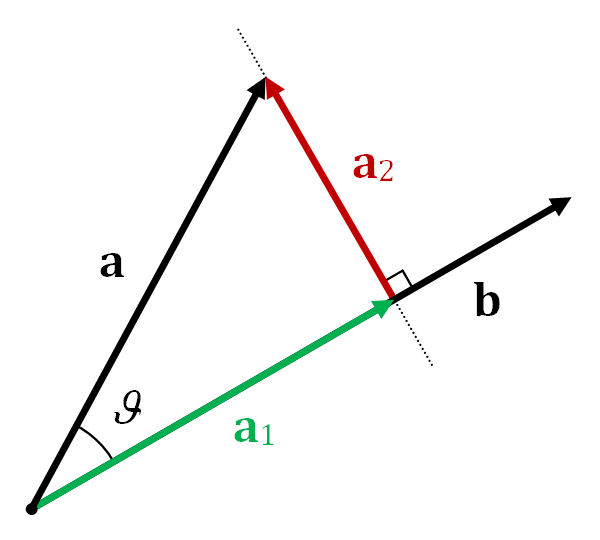
\includegraphics[width=0.5\textwidth]{images/projection.png}
    \end{center}

    \begin{equation}
        \vec{a}_1 = \frac{\langle \vec{a}, \vec{b} \rangle}{\|b\|^2} \vec{b}
    \end{equation}
\end{frame}

\begin{frame}
    \frametitle{Gram-Schmidt}

    \begin{align}
        \vec{q}_1 &= \frac{\vec{s}_1}{\|\vec{s}_1\|} \\
        \vec{e}_i &= \vec{s}_i - \sum_{k = 1}^{i - 1} \langle s_i, q_k \rangle q_k \\
        \vec{q}_i &= \frac{\vec{e}_i}{\|\vec{e}_i\|}
    \end{align}
\end{frame}

\begin{frame}
    \frametitle{GS True or False}

    \begin{itemize}
        \item You can perform GS with the \(\vec{s}\) vectors in any order. \pause{\textbf{True}}
        \item Gram-Schmidt changes the span of the basis vectors. \pause{\textbf{False}}
    \end{itemize}
\end{frame}
